\biohead{Frank Bertram Hussey}{During the war.\cite{CaptainHusseyDisplay}}

Frank Hussey was born on 26 April 1908 in Toodyay\cite{RaeWestAus} to Dr~Bertram Hussey and his wife.\cite{WesternMail1936}
Dr~Hussey died some time before 1936.\cite{MilitaryWedding}

He attended Guildford Grammar School 1920--1923\cite{FBHguildford}
and then Duntroon (when it was in Melbourne).\cite{RaeWestAus}

In the lead-up to the \idx{Second World War} he was seconded from the Army to oversee the construction of the railway on Rottnest
(from Kingston Barracks to Oliver Hill).\cite{RaeWestAus}

On Tuesday 3 March 1936 he married Hilda McCue (of Rockdale NSW\cite{WestAus1936p4})
in the hotel on Rottnest.\cite{WestAus1936p19}
They were married in the Music Room.\cite{MilitaryWedding}
Captain K. Hall was the chairman at the reception.\cite{MilitaryWedding}
Hilda cut the cake with Frank's military sword.\cite{MilitaryWedding}

He rose to the rank of Brigadier during WW2,\cite{FBHwar}
and was discharged from the Army in 1958.\cite{CaptainHusseyDisplay}

After the war, he married Rae (\p{Lilian_Rae_Wilson}). Together they lived in Wyndham,
where from 1960 to `63 he was an engineer on the Ord River Diversion Dam.

Frank died on 11 May 1985 at Hollywood Hospital in Perth.

In November 2003 a new railcar on the tourist railway on Rottnest was named \emph{Captain Hussey} in his honour (see Fig.~\ref{CaptainHussey}).\cite{RIA2004}
An information notice at the Settlement railway station read as follows:\cite{CaptainHusseyDisplay}

\begin{quotation}
\begin{center}
\textbf{Brigadier B.F. (Frank) Hussey (1907--1985)}
\end{center}

In 1933 as an Engineer Adviser, Frank Hussey joined General Sir Talbot Hobbs, Colonel Whitelaw and Major Payne on a reconnaissance of Rottnest Island to select sites for military installations.

Captain Hussey was to return to March 1935 as Engineer-in-Charge on Rottnest Island for the Department of the Interior. Despite this grant title, all the Army provided him with when he first arrived was two horses, a groom and a batman (a military term for an officer's servant).

He was reponsible for carrying out the preliminary work for all the military sites on the Island and in particular to supervise the construction of the railway from the Army Jetty to Bickley and Oliver Hill.

In an interview recorded in 1981, Frank Hussey described some of the challenges they had to overcome in constructing extensions to the railway line:

\emph{``A very large problem was to stop the embankments blowing away\dots what we did was ped down lots of ti-tree, and after trying various other things we found that by far the best thing was the Rottnest Daisy, to get that growing on the banks.''}

He left Rottnest Island at the end of 1937 and served in New Guinea during World War II. Frank Hussey held the rank of Captain while stationed on Rottnest Island, but reached the rank of Brigadier by the time he was discharged from the Army in 1958.
\end{quotation}

\begin{figure}
 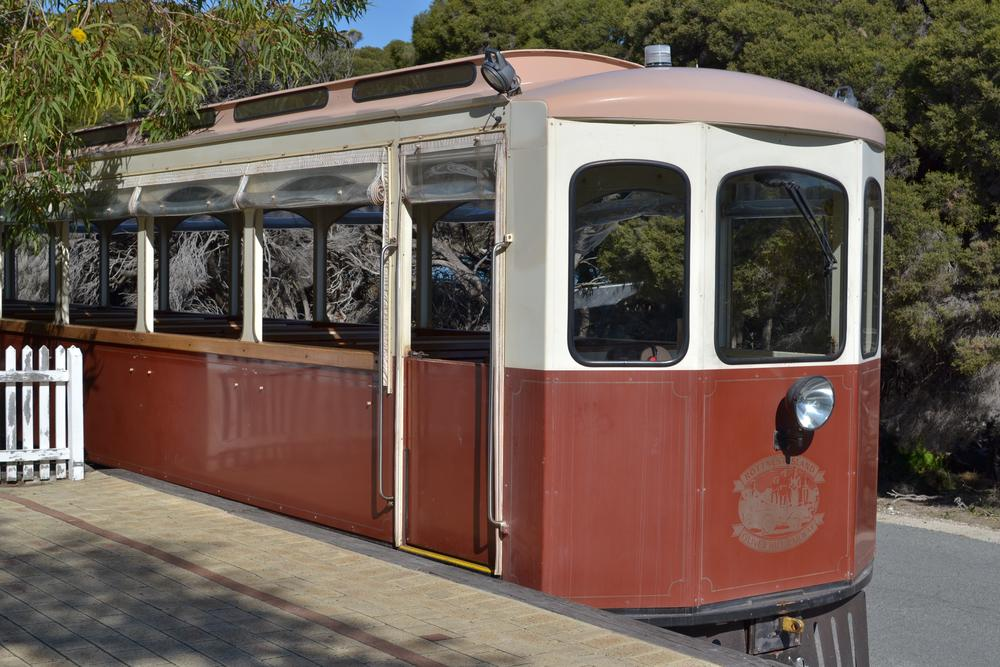
\includegraphics[width=\textwidth]{photos/Captain_Hussey}
 \caption{\emph{Captain Hussey} at the Settlement railway station, May 2015.\cite{CaptainHusseyPhoto}}
 \label{CaptainHussey}
\end{figure}
